% generated by Plantuml 1.2022.7       
\definecolor{plantucolor0000}{RGB}{255,255,255}
\definecolor{plantucolor0001}{RGB}{24,24,24}
\definecolor{plantucolor0002}{RGB}{0,0,0}
\definecolor{plantucolor0003}{RGB}{226,226,240}
\definecolor{plantucolor0004}{RGB}{238,238,238}
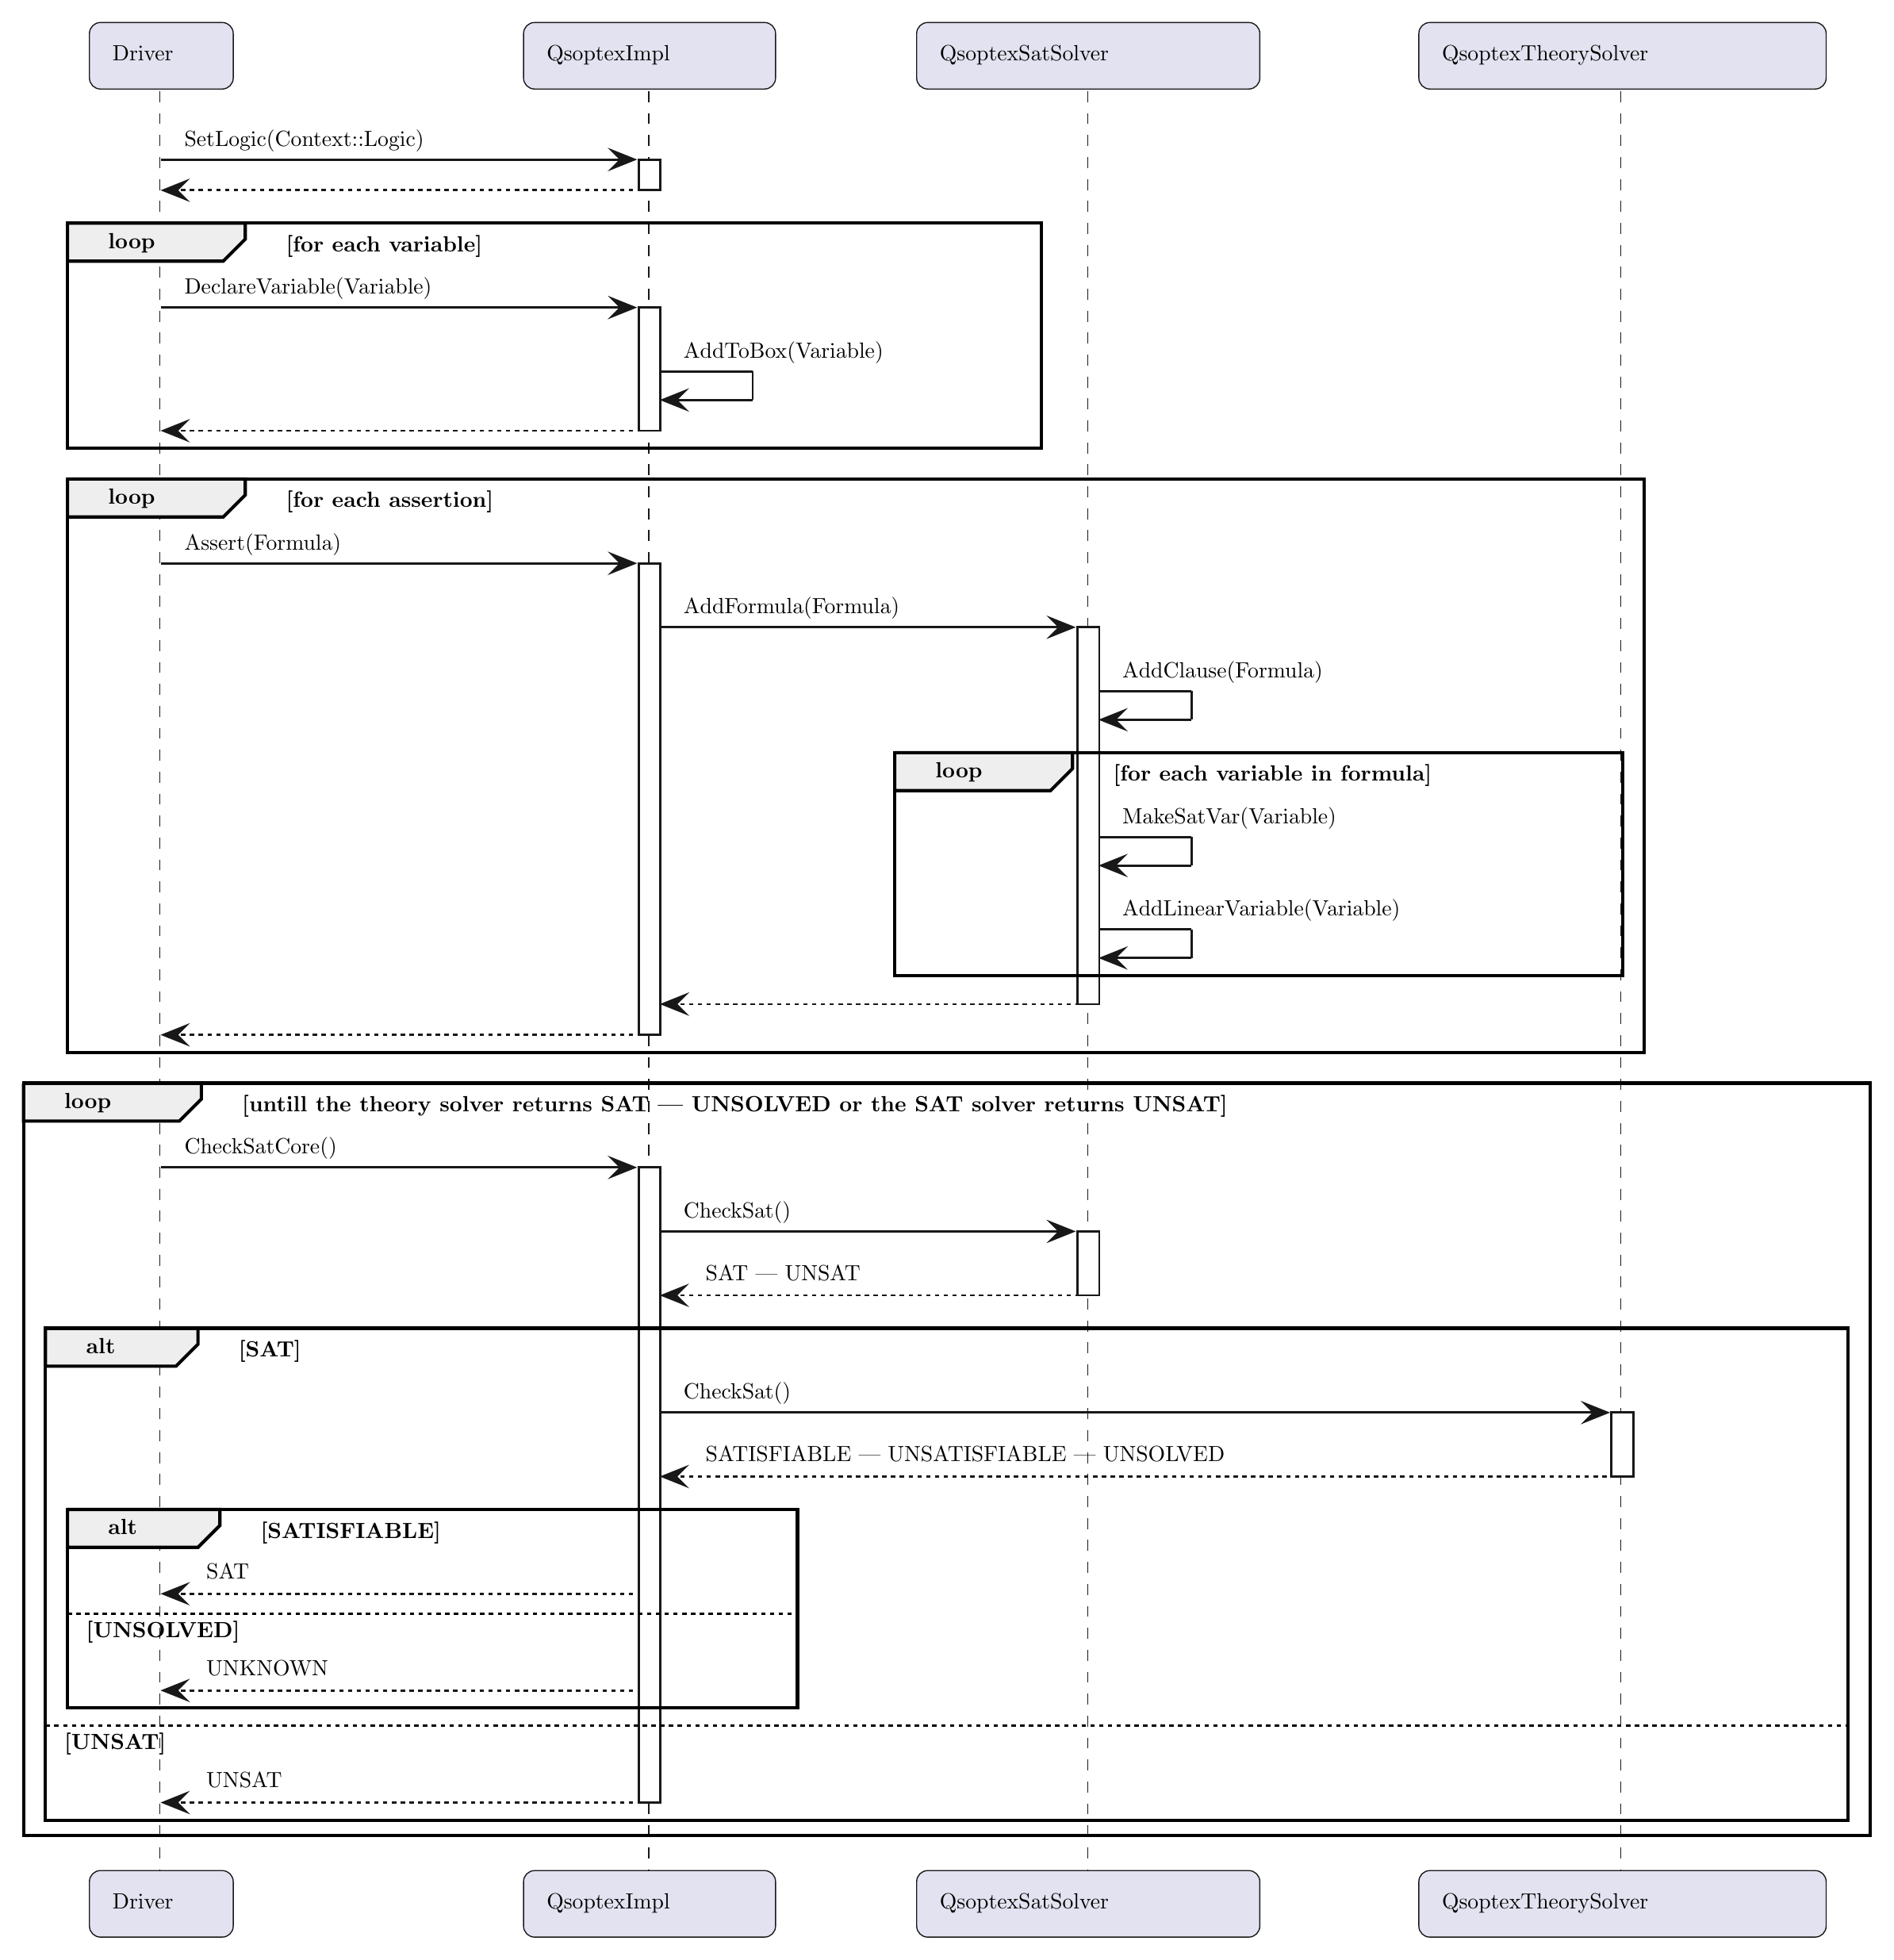
\begin{tikzpicture}[yscale=-1
,pstyle0/.style={color=plantucolor0001,fill=white,line width=1.0pt}
,pstyle1/.style={color=black,line width=1.5pt}
,pstyle2/.style={color=plantucolor0001,line width=0.5pt,dash pattern=on 5.0pt off 5.0pt}
,pstyle3/.style={color=plantucolor0001,fill=plantucolor0003,line width=0.5pt}
,pstyle4/.style={color=plantucolor0001,fill=plantucolor0001,line width=1.0pt}
,pstyle5/.style={color=plantucolor0001,line width=1.0pt}
,pstyle6/.style={color=plantucolor0001,line width=1.0pt,dash pattern=on 2.0pt off 2.0pt}
,pstyle7/.style={color=black,fill=plantucolor0004,line width=1.5pt}
,pstyle8/.style={color=black,line width=1.0pt,dash pattern=on 2.0pt off 2.0pt}
]
\draw[pstyle0] (290.1889pt,67.4297pt) rectangle (300.1889pt,81.4297pt);
\draw[pstyle0] (290.1889pt,134.835pt) rectangle (300.1889pt,190.9678pt);
\draw[pstyle0] (290.1889pt,251.373pt) rectangle (300.1889pt,466.1768pt);
\draw[pstyle0] (290.1889pt,526.582pt) rectangle (300.1889pt,815.9023pt);
\draw[pstyle0] (490.0441pt,280.5059pt) rectangle (500.0441pt,452.1768pt);
\draw[pstyle0] (490.0441pt,555.7148pt) rectangle (500.0441pt,584.8477pt);
\draw[pstyle0] (733.4495pt,638.2529pt) rectangle (743.4495pt,667.3857pt);
\draw[pstyle1] (30pt,96.4297pt) rectangle (473.824pt,198.9678pt);
\draw[pstyle1] (30pt,212.9678pt) rectangle (748.4495pt,474.1768pt);
\draw[pstyle1] (406.8841pt,337.6387pt) rectangle (738.4495pt,439.1768pt);
\draw[pstyle1] (10pt,488.1768pt) rectangle (851.2283pt,830.9023pt);
\draw[pstyle1] (20pt,599.8477pt) rectangle (841.2283pt,823.9023pt);
\draw[pstyle1] (30pt,682.3857pt) rectangle (362.5889pt,772.8467pt);
\draw[pstyle2] (72pt,36.2969pt) -- (72pt,847.9023pt);
\draw[pstyle2] (294.7889pt,36.2969pt) -- (294.7889pt,847.9023pt);
\draw[pstyle2] (494.8841pt,36.2969pt) -- (494.8841pt,847.9023pt);
\draw[pstyle2] (737.6707pt,36.2969pt) -- (737.6707pt,847.9023pt);
\draw[pstyle3] (40pt,10pt) arc (180:270:5pt) -- (45pt,5pt) -- (100.5111pt,5pt) arc (270:360:5pt) -- (105.5111pt,10pt) -- (105.5111pt,30.2969pt) arc (0:90:5pt) -- (100.5111pt,35.2969pt) -- (45pt,35.2969pt) arc (90:180:5pt) -- (40pt,30.2969pt) -- cycle;
\node at (47pt,12pt)[below right,color=black]{Driver};
\draw[pstyle3] (40pt,851.9023pt) arc (180:270:5pt) -- (45pt,846.9023pt) -- (100.5111pt,846.9023pt) arc (270:360:5pt) -- (105.5111pt,851.9023pt) -- (105.5111pt,872.1992pt) arc (0:90:5pt) -- (100.5111pt,877.1992pt) -- (45pt,877.1992pt) arc (90:180:5pt) -- (40pt,872.1992pt) -- cycle;
\node at (47pt,853.9023pt)[below right,color=black]{Driver};
\draw[pstyle3] (237.7889pt,10pt) arc (180:270:5pt) -- (242.7889pt,5pt) -- (347.5889pt,5pt) arc (270:360:5pt) -- (352.5889pt,10pt) -- (352.5889pt,30.2969pt) arc (0:90:5pt) -- (347.5889pt,35.2969pt) -- (242.7889pt,35.2969pt) arc (90:180:5pt) -- (237.7889pt,30.2969pt) -- cycle;
\node at (244.7889pt,12pt)[below right,color=black]{QsoptexImpl};
\draw[pstyle3] (237.7889pt,851.9023pt) arc (180:270:5pt) -- (242.7889pt,846.9023pt) -- (347.5889pt,846.9023pt) arc (270:360:5pt) -- (352.5889pt,851.9023pt) -- (352.5889pt,872.1992pt) arc (0:90:5pt) -- (347.5889pt,877.1992pt) -- (242.7889pt,877.1992pt) arc (90:180:5pt) -- (237.7889pt,872.1992pt) -- cycle;
\node at (244.7889pt,853.9023pt)[below right,color=black]{QsoptexImpl};
\draw[pstyle3] (416.8841pt,10pt) arc (180:270:5pt) -- (421.8841pt,5pt) -- (568.2041pt,5pt) arc (270:360:5pt) -- (573.2041pt,10pt) -- (573.2041pt,30.2969pt) arc (0:90:5pt) -- (568.2041pt,35.2969pt) -- (421.8841pt,35.2969pt) arc (90:180:5pt) -- (416.8841pt,30.2969pt) -- cycle;
\node at (423.8841pt,12pt)[below right,color=black]{QsoptexSatSolver};
\draw[pstyle3] (416.8841pt,851.9023pt) arc (180:270:5pt) -- (421.8841pt,846.9023pt) -- (568.2041pt,846.9023pt) arc (270:360:5pt) -- (573.2041pt,851.9023pt) -- (573.2041pt,872.1992pt) arc (0:90:5pt) -- (568.2041pt,877.1992pt) -- (421.8841pt,877.1992pt) arc (90:180:5pt) -- (416.8841pt,872.1992pt) -- cycle;
\node at (423.8841pt,853.9023pt)[below right,color=black]{QsoptexSatSolver};
\draw[pstyle3] (645.6707pt,10pt) arc (180:270:5pt) -- (650.6707pt,5pt) -- (826.2283pt,5pt) arc (270:360:5pt) -- (831.2283pt,10pt) -- (831.2283pt,30.2969pt) arc (0:90:5pt) -- (826.2283pt,35.2969pt) -- (650.6707pt,35.2969pt) arc (90:180:5pt) -- (645.6707pt,30.2969pt) -- cycle;
\node at (652.6707pt,12pt)[below right,color=black]{QsoptexTheorySolver};
\draw[pstyle3] (645.6707pt,851.9023pt) arc (180:270:5pt) -- (650.6707pt,846.9023pt) -- (826.2283pt,846.9023pt) arc (270:360:5pt) -- (831.2283pt,851.9023pt) -- (831.2283pt,872.1992pt) arc (0:90:5pt) -- (826.2283pt,877.1992pt) -- (650.6707pt,877.1992pt) arc (90:180:5pt) -- (645.6707pt,872.1992pt) -- cycle;
\node at (652.6707pt,853.9023pt)[below right,color=black]{QsoptexTheorySolver};
\draw[pstyle0] (290.1889pt,67.4297pt) rectangle (300.1889pt,81.4297pt);
\draw[pstyle0] (290.1889pt,134.835pt) rectangle (300.1889pt,190.9678pt);
\draw[pstyle0] (290.1889pt,251.373pt) rectangle (300.1889pt,466.1768pt);
\draw[pstyle0] (290.1889pt,526.582pt) rectangle (300.1889pt,815.9023pt);
\draw[pstyle0] (490.0441pt,280.5059pt) rectangle (500.0441pt,452.1768pt);
\draw[pstyle0] (490.0441pt,555.7148pt) rectangle (500.0441pt,584.8477pt);
\draw[pstyle0] (733.4495pt,638.2529pt) rectangle (743.4495pt,667.3857pt);
\draw[pstyle4] (278.1889pt,63.4297pt) -- (288.1889pt,67.4297pt) -- (278.1889pt,71.4297pt) -- (282.1889pt,67.4297pt) -- cycle;
\draw[pstyle5] (72.7556pt,67.4297pt) -- (284.1889pt,67.4297pt);
\node at (79.7556pt,50.2969pt)[below right,color=black]{SetLogic(Context::Logic)};
\draw[pstyle4] (83.7556pt,77.4297pt) -- (73.7556pt,81.4297pt) -- (83.7556pt,85.4297pt) -- (79.7556pt,81.4297pt) -- cycle;
\draw[pstyle6] (77.7556pt,81.4297pt) -- (294.1889pt,81.4297pt);
\draw[pstyle7] (30pt,96.4297pt) -- (111pt,96.4297pt) -- (111pt,103.7021pt) -- (101pt,113.7021pt) -- (30pt,113.7021pt) -- (30pt,96.4297pt);
\draw[pstyle1] (30pt,96.4297pt) rectangle (473.824pt,198.9678pt);
\node at (45pt,97.4297pt)[below right,color=black]{\textbf{loop}};
\node at (126pt,98.4297pt)[below right,color=black]{\textbf{[for each variable]}};
\draw[pstyle4] (278.1889pt,130.835pt) -- (288.1889pt,134.835pt) -- (278.1889pt,138.835pt) -- (282.1889pt,134.835pt) -- cycle;
\draw[pstyle5] (72.7556pt,134.835pt) -- (284.1889pt,134.835pt);
\node at (79.7556pt,117.7021pt)[below right,color=black]{DeclareVariable(Variable)};
\draw[pstyle5] (300.1889pt,163.9678pt) -- (342.1889pt,163.9678pt);
\draw[pstyle5] (342.1889pt,163.9678pt) -- (342.1889pt,176.9678pt);
\draw[pstyle5] (301.1889pt,176.9678pt) -- (342.1889pt,176.9678pt);
\draw[pstyle4] (311.1889pt,172.9678pt) -- (301.1889pt,176.9678pt) -- (311.1889pt,180.9678pt) -- (307.1889pt,176.9678pt) -- cycle;
\node at (307.1889pt,146.835pt)[below right,color=black]{AddToBox(Variable)};
\draw[pstyle4] (83.7556pt,186.9678pt) -- (73.7556pt,190.9678pt) -- (83.7556pt,194.9678pt) -- (79.7556pt,190.9678pt) -- cycle;
\draw[pstyle6] (77.7556pt,190.9678pt) -- (294.1889pt,190.9678pt);
\draw[pstyle7] (30pt,212.9678pt) -- (111pt,212.9678pt) -- (111pt,220.2402pt) -- (101pt,230.2402pt) -- (30pt,230.2402pt) -- (30pt,212.9678pt);
\draw[pstyle1] (30pt,212.9678pt) rectangle (748.4495pt,474.1768pt);
\node at (45pt,213.9678pt)[below right,color=black]{\textbf{loop}};
\node at (126pt,214.9678pt)[below right,color=black]{\textbf{[for each assertion]}};
\draw[pstyle4] (278.1889pt,247.373pt) -- (288.1889pt,251.373pt) -- (278.1889pt,255.373pt) -- (282.1889pt,251.373pt) -- cycle;
\draw[pstyle5] (72.7556pt,251.373pt) -- (284.1889pt,251.373pt);
\node at (79.7556pt,234.2402pt)[below right,color=black]{Assert(Formula)};
\draw[pstyle4] (478.0441pt,276.5059pt) -- (488.0441pt,280.5059pt) -- (478.0441pt,284.5059pt) -- (482.0441pt,280.5059pt) -- cycle;
\draw[pstyle5] (300.1889pt,280.5059pt) -- (484.0441pt,280.5059pt);
\node at (307.1889pt,263.373pt)[below right,color=black]{AddFormula(Formula)};
\draw[pstyle5] (500.0441pt,309.6387pt) -- (542.0441pt,309.6387pt);
\draw[pstyle5] (542.0441pt,309.6387pt) -- (542.0441pt,322.6387pt);
\draw[pstyle5] (501.0441pt,322.6387pt) -- (542.0441pt,322.6387pt);
\draw[pstyle4] (511.0441pt,318.6387pt) -- (501.0441pt,322.6387pt) -- (511.0441pt,326.6387pt) -- (507.0441pt,322.6387pt) -- cycle;
\node at (507.0441pt,292.5059pt)[below right,color=black]{AddClause(Formula)};
\draw[pstyle7] (406.8841pt,337.6387pt) -- (487.8841pt,337.6387pt) -- (487.8841pt,344.9111pt) -- (477.8841pt,354.9111pt) -- (406.8841pt,354.9111pt) -- (406.8841pt,337.6387pt);
\draw[pstyle1] (406.8841pt,337.6387pt) rectangle (738.4495pt,439.1768pt);
\node at (421.8841pt,338.6387pt)[below right,color=black]{\textbf{loop}};
\node at (502.8841pt,339.6387pt)[below right,color=black]{\textbf{[for each variable in formula]}};
\draw[pstyle5] (500.0441pt,376.0439pt) -- (542.0441pt,376.0439pt);
\draw[pstyle5] (542.0441pt,376.0439pt) -- (542.0441pt,389.0439pt);
\draw[pstyle5] (501.0441pt,389.0439pt) -- (542.0441pt,389.0439pt);
\draw[pstyle4] (511.0441pt,385.0439pt) -- (501.0441pt,389.0439pt) -- (511.0441pt,393.0439pt) -- (507.0441pt,389.0439pt) -- cycle;
\node at (507.0441pt,358.9111pt)[below right,color=black]{MakeSatVar(Variable)};
\draw[pstyle5] (500.0441pt,418.1768pt) -- (542.0441pt,418.1768pt);
\draw[pstyle5] (542.0441pt,418.1768pt) -- (542.0441pt,431.1768pt);
\draw[pstyle5] (501.0441pt,431.1768pt) -- (542.0441pt,431.1768pt);
\draw[pstyle4] (511.0441pt,427.1768pt) -- (501.0441pt,431.1768pt) -- (511.0441pt,435.1768pt) -- (507.0441pt,431.1768pt) -- cycle;
\node at (507.0441pt,401.0439pt)[below right,color=black]{AddLinearVariable(Variable)};
\draw[pstyle4] (311.1889pt,448.1768pt) -- (301.1889pt,452.1768pt) -- (311.1889pt,456.1768pt) -- (307.1889pt,452.1768pt) -- cycle;
\draw[pstyle6] (305.1889pt,452.1768pt) -- (494.0441pt,452.1768pt);
\draw[pstyle4] (83.7556pt,462.1768pt) -- (73.7556pt,466.1768pt) -- (83.7556pt,470.1768pt) -- (79.7556pt,466.1768pt) -- cycle;
\draw[pstyle6] (77.7556pt,466.1768pt) -- (294.1889pt,466.1768pt);
\draw[pstyle7] (10pt,488.1768pt) -- (91pt,488.1768pt) -- (91pt,495.4492pt) -- (81pt,505.4492pt) -- (10pt,505.4492pt) -- (10pt,488.1768pt);
\draw[pstyle1] (10pt,488.1768pt) rectangle (851.2283pt,830.9023pt);
\node at (25pt,489.1768pt)[below right,color=black]{\textbf{loop}};
\node at (106pt,490.1768pt)[below right,color=black]{\textbf{[untill the theory solver returns SAT | UNSOLVED or the SAT solver returns UNSAT]}};
\draw[pstyle4] (278.1889pt,522.582pt) -- (288.1889pt,526.582pt) -- (278.1889pt,530.582pt) -- (282.1889pt,526.582pt) -- cycle;
\draw[pstyle5] (72.7556pt,526.582pt) -- (284.1889pt,526.582pt);
\node at (79.7556pt,509.4492pt)[below right,color=black]{CheckSatCore()};
\draw[pstyle4] (478.0441pt,551.7148pt) -- (488.0441pt,555.7148pt) -- (478.0441pt,559.7148pt) -- (482.0441pt,555.7148pt) -- cycle;
\draw[pstyle5] (300.1889pt,555.7148pt) -- (484.0441pt,555.7148pt);
\node at (307.1889pt,538.582pt)[below right,color=black]{CheckSat()};
\draw[pstyle4] (311.1889pt,580.8477pt) -- (301.1889pt,584.8477pt) -- (311.1889pt,588.8477pt) -- (307.1889pt,584.8477pt) -- cycle;
\draw[pstyle6] (305.1889pt,584.8477pt) -- (494.0441pt,584.8477pt);
\node at (317.1889pt,567.7148pt)[below right,color=black]{SAT | UNSAT};
\draw[pstyle7] (20pt,599.8477pt) -- (89.4381pt,599.8477pt) -- (89.4381pt,607.1201pt) -- (79.4381pt,617.1201pt) -- (20pt,617.1201pt) -- (20pt,599.8477pt);
\draw[pstyle1] (20pt,599.8477pt) rectangle (841.2283pt,823.9023pt);
\node at (35pt,600.8477pt)[below right,color=black]{\textbf{alt}};
\node at (104.4381pt,601.8477pt)[below right,color=black]{\textbf{[SAT]}};
\draw[pstyle4] (721.4495pt,634.2529pt) -- (731.4495pt,638.2529pt) -- (721.4495pt,642.2529pt) -- (725.4495pt,638.2529pt) -- cycle;
\draw[pstyle5] (300.1889pt,638.2529pt) -- (727.4495pt,638.2529pt);
\node at (307.1889pt,621.1201pt)[below right,color=black]{CheckSat()};
\draw[pstyle4] (311.1889pt,663.3857pt) -- (301.1889pt,667.3857pt) -- (311.1889pt,671.3857pt) -- (307.1889pt,667.3857pt) -- cycle;
\draw[pstyle6] (305.1889pt,667.3857pt) -- (737.4495pt,667.3857pt);
\node at (317.1889pt,650.2529pt)[below right,color=black]{SATISFIABLE | UNSATISFIABLE | UNSOLVED};
\draw[pstyle7] (30pt,682.3857pt) -- (99.4381pt,682.3857pt) -- (99.4381pt,689.6582pt) -- (89.4381pt,699.6582pt) -- (30pt,699.6582pt) -- (30pt,682.3857pt);
\draw[pstyle1] (30pt,682.3857pt) rectangle (362.5889pt,772.8467pt);
\node at (45pt,683.3857pt)[below right,color=black]{\textbf{alt}};
\node at (114.4381pt,684.3857pt)[below right,color=black]{\textbf{[SATISFIABLE]}};
\draw[pstyle4] (83.7556pt,716.791pt) -- (73.7556pt,720.791pt) -- (83.7556pt,724.791pt) -- (79.7556pt,720.791pt) -- cycle;
\draw[pstyle6] (77.7556pt,720.791pt) -- (289.1889pt,720.791pt);
\node at (89.7556pt,703.6582pt)[below right,color=black]{SAT};
\draw[pstyle8] (30pt,729.791pt) -- (362.5889pt,729.791pt);
\node at (35pt,729.791pt)[below right,color=black]{\textbf{[UNSOLVED]}};
\draw[pstyle4] (83.7556pt,760.8467pt) -- (73.7556pt,764.8467pt) -- (83.7556pt,768.8467pt) -- (79.7556pt,764.8467pt) -- cycle;
\draw[pstyle6] (77.7556pt,764.8467pt) -- (289.1889pt,764.8467pt);
\node at (89.7556pt,747.7139pt)[below right,color=black]{UNKNOWN};
\draw[pstyle8] (20pt,780.8467pt) -- (841.2283pt,780.8467pt);
\node at (25pt,780.8467pt)[below right,color=black]{\textbf{[UNSAT]}};
\draw[pstyle4] (83.7556pt,811.9023pt) -- (73.7556pt,815.9023pt) -- (83.7556pt,819.9023pt) -- (79.7556pt,815.9023pt) -- cycle;
\draw[pstyle6] (77.7556pt,815.9023pt) -- (294.1889pt,815.9023pt);
\node at (89.7556pt,798.7695pt)[below right,color=black]{UNSAT};
\end{tikzpicture}
